\chapter{Revisión de técnicas}

En este capítulo se describen los procesos y algoritmos utilizados a lo largo del trabajo descrito en esta memoria. Concretamente, se explica el concepto de la \textbf{ciencia de datos} y su ciclo de vida, detallando los conceptos principales en cada una de las etapas del proceso. Tras esto, se estudian los modelos de regresión utilizados durante el trabajo - con especial énfasis en los modelos de \textit{ensembles} basados en técnicas de \textit{\textbf{Gradient Boosting}}.

\section{Ciencia de datos y el ciclo de vida de los datos}

La \textbf{ciencia de datos} es el estudio de la extracción de conocimiento útil a partir de datos, y de la generalización de dicho proceso a cualquier problema \cite{Donoho02102017}. Dicho proceso incluye la recolección y almacenamiento, mantenimiento, procesamiento, análisis y visualización de enormes cantidades de datos heterogéneos - asociados a un gran abanico de aplicaciones y dominios en muchas ocasiones multidisciplinarios \cite{10.1145/2500499}.

Desde su origen, la ciencia de datos ha evolucionado como un campo interdisciplinar que integra conocimientos y técnicas de otras disciplinas afines como el análisis de datos, la estadística o la minería de datos \cite{potential}. Ahora bien, la principal diferencia con estos campos se encuentra en el fin: el aprendizaje a partir de los datos \cite{Donoho02102017} y la capacidad de adquirir nuevo conocimiento capaz de ser utilizado para la toma de decisiones y la predicción \cite{10.1145/2500499}.

\begin{figure}[h]
	\centering
	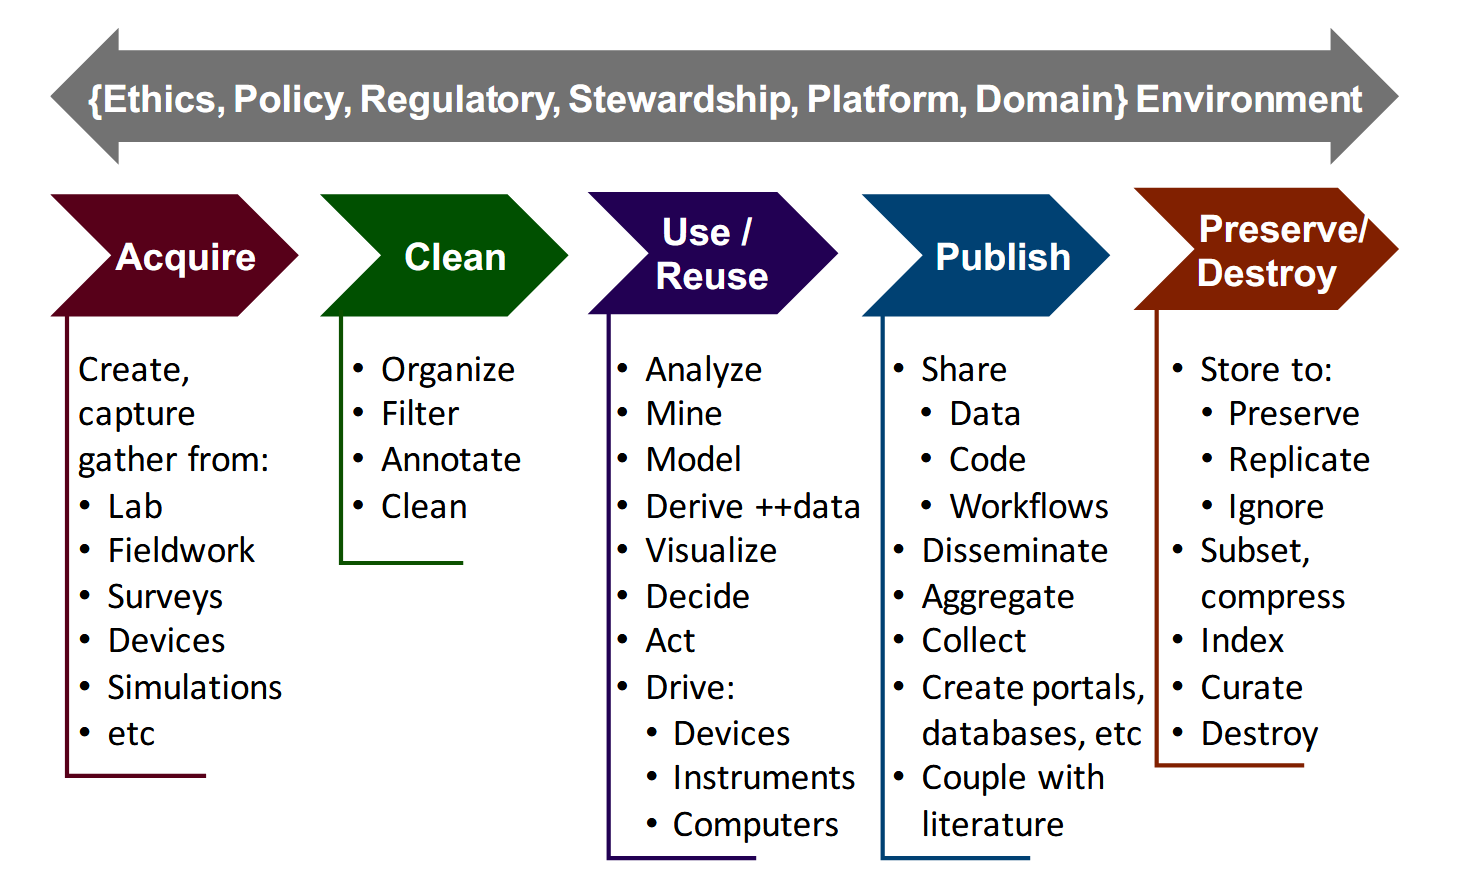
\includegraphics[width=0.8\linewidth]{figs/chapter2/datalifecycle}
	\caption{Ciclo de vida de los datos \cite{potential}}
	\label{fig:datalifecycle}
\end{figure}

Por definición, la ciencia de datos depende completamente de los datos sobre los que se trabajan. Por esto, los ciclos de vida de la ciencia de datos dependen generalmente del \textbf{ciclo de vida de los datos}: las distintas etapas por las que pasa un conjunto de datos desde su recolección e investigación hasta su uso final \cite{datasciencelifecycle}. Como se observa en la \textbf{Figura \ref{fig:datalifecycle}}, este ciclo está tradicionalmente dividido en \textbf{cinco} apartados \cite{potential}:

\begin{enumerate}
	\item \textbf{Adquisición:} En la actualidad, los datos se generan en cantidades masivas - del orden de \textbf{exabytes por hora} \cite{Wing2019Data}. Por tanto, el primer paso del ciclo consiste en la adquisición y almacenamiento eficiente de los datos necesarios para el proceso.
	\item \textbf{Limpieza:} Tras la adquisición, el segundo paso del ciclo consiste en la transformación de los datos originales en datos utilizables posteriormente - a través de procesos de limpieza, imputación, formateo...
	\item \textbf{Uso y re-uso:}  El tercer paso del ciclo consiste en el uso de los datos procesados con el fin de adquirir conocimiento y tomar decisiones a partir de éstos. Éste apartado se puede dividir, a su vez, en tres subapartados \cite{Wing2019Data}:
		\begin{enumerate}
			\item \textbf{Análisis exploratorio:} El estudio del comportamiento de los datos con el fin de plantear hipótesis para guiar el resto del ciclo de datos \cite{eda}.
			\item \textbf{Modelado:} El uso de técnicas computacionales y estadísticas para extraer conocimiento y predicciones a partir del conjunto de datos.
			\item \textbf{Visualización, interpretación y actuación:}  La representación gráfica de los resultados del uso de los datos, con el fin de facilitar la toma de decisiones posterior a las personas.
		\end{enumerate}
	\item \textbf{Publicación:} El cuarto paso del ciclo consiste en la diseminación de los resultados del proceso - con el fin de que el conocimiento creado pueda ser conocido y reutilizado por el mayor número de personas posible.
	\item \textbf{Preservación o destrucción:} El quinto y último paso del ciclo consiste en la preservación o destrucción de los datos utilizados - cumpliendo con otros factores como pueden ser las consideraciones éticas o regulatorias.
\end{enumerate}



\subsection{CRISP-DM: Cross-Industry Standard Process for Data Mining}

\begin{figure}[h]
	\centering
	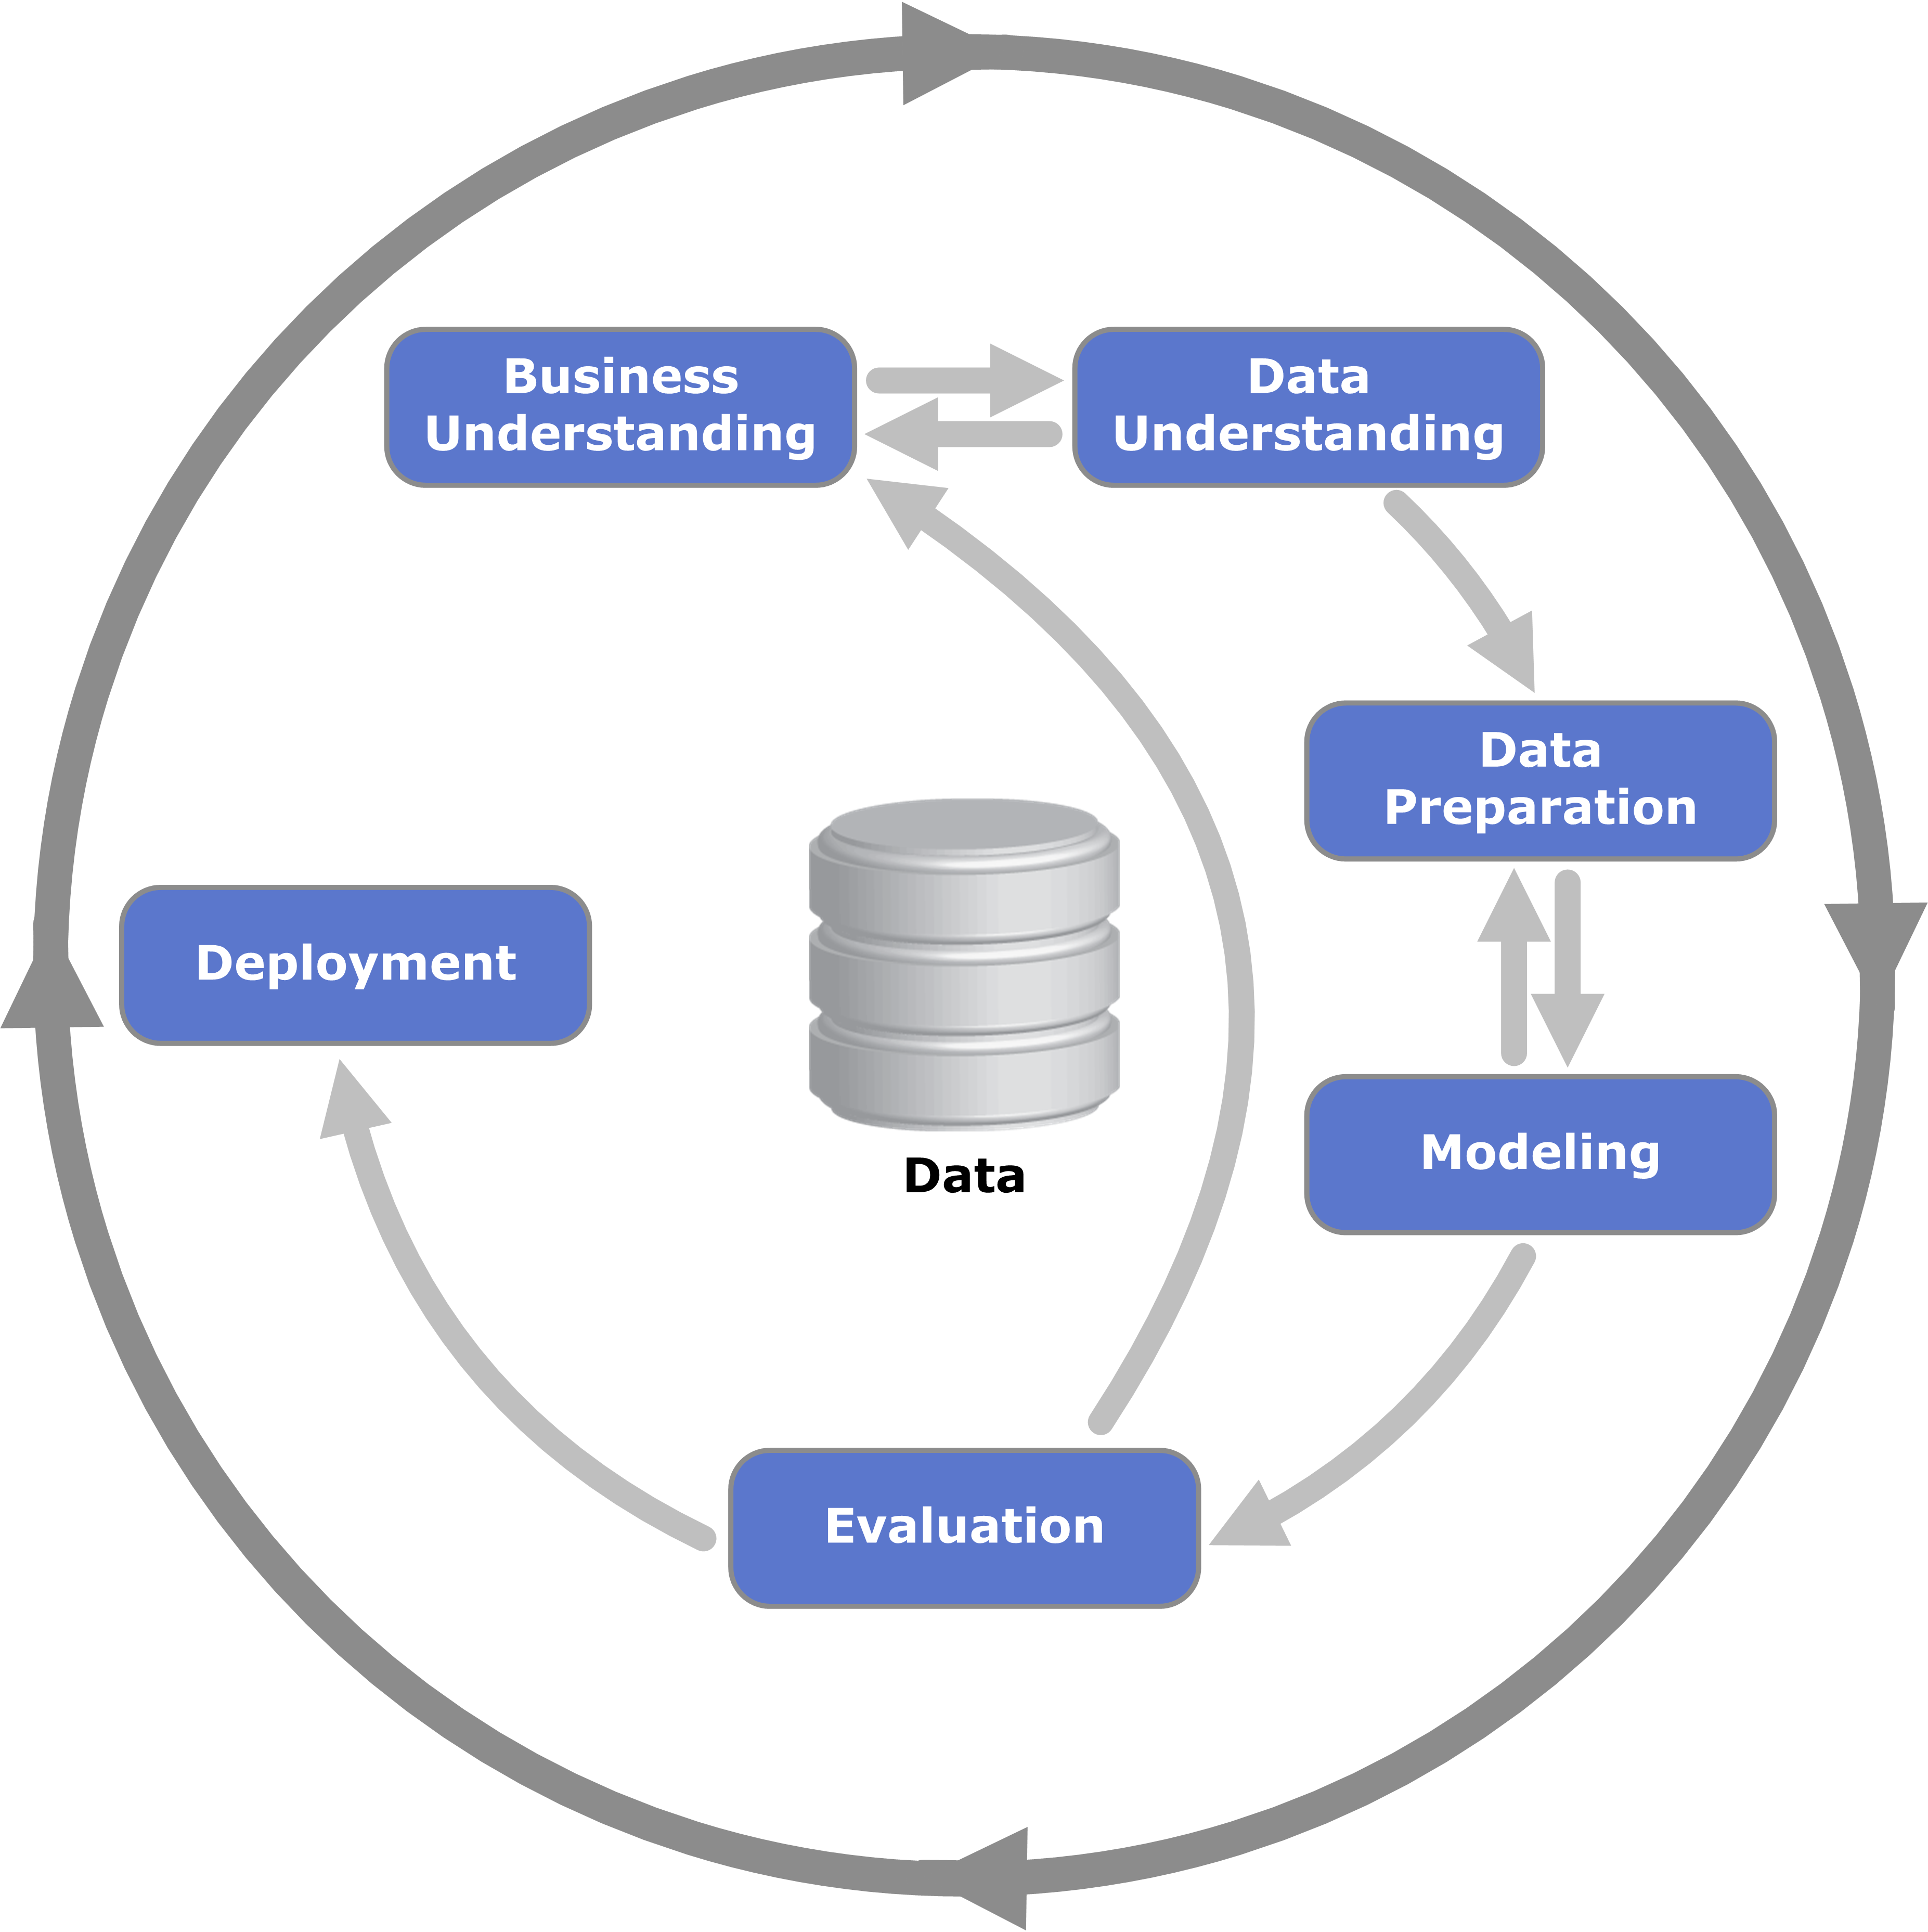
\includegraphics[width=0.6\linewidth]{figs/chapter2/crispdm}
	\caption{Ciclo de vida de la ciencia de datos según CRISP-DM \cite{shearer2000crisp}}
	\label{fig:crispdm}
\end{figure}


\section{Aprendizaje supervisado y modelos de regresión}

\subsection{Modelos simples}

\subsubsection{Modelos de regresión lineal}

\subsubsection{Árboles de decisión}

\subsubsection{Máquinas de vectores de soporte}

\subsection{Modelos grupales - Ensembles}

\subsubsection{Bagging}

\subsubsection{Boosting}

\subsubsection{Gradient Boosting}